\label{chap:eeg}
Für das Projekt wurde ein EMOTIV Epoc+ EEG Headset \footnote{\url{http://emotiv.com/epoc}} (Abb. \ref{fig:eeg}, Quellen \footnote{\url{https://en.wikipedia.org/wiki/Electroencephalography\#/media/File:EEG_cap.jpg}} \footnote{\url{http://emotiv.com/wp-content/uploads/2016/04/epoc_hero_01_flipped.png}}) verwendet. Es besitzt 14 EEG Kanäle, sowie ein Gyroskop und sendet seine Daten via Bluetooth an den Rechner. Das Headset wird über den Kopf gestülpt und besitzen an den Sensorenden einen Filz der mit Kochsalzlösung befeuchtet wird. Das gesamte Headset wird einfach über den Kopf gestülpt.

\begin{figure}[h] 
  \begin{center}
    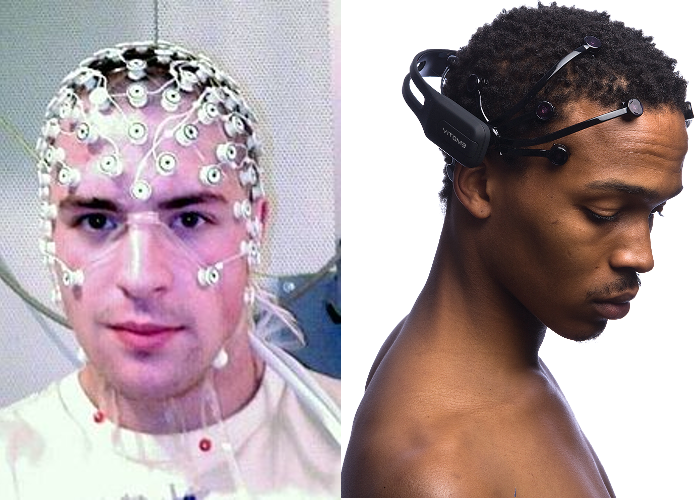
\includegraphics[width=0.75\columnwidth]{eeg}
    \caption[Medzinisches EEG / EMOTIV Epoc+]{Links: Ein medizinisches EEG mit 64 Kanälen. Rechts: Das EMOTIV Epoc+ EEG Headset mit 14 Kanälen.\label{fig:eeg}}
  \end{center}
\end{figure}

Die Sensoranordnung ist an das internationale 10-20 System \cite{10-20}  angelehnt (\ref{fig:epoc_sensors}). Hierbei handelt es sich um eine standardisierte relative Anordnung der Elektroden. Die Rohdaten werden Abtastrate von 128Hz geliefert und enthalten neben dem Wert auch die Signalstärke (Qualität). Leider liefert die mitgelieferte SDK die Rohdaten nicht in Echtzeit, weshalb die Open-Source Lösung Emokit\footnote{\url{https://github.com/openyou/emokit}} eingebunden wurde.

\begin{figure}[h] 
  \begin{center}
    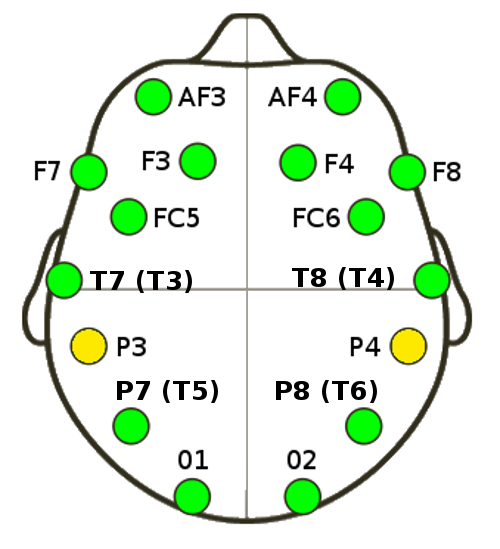
\includegraphics[width=0.5\columnwidth]{epoc_sensors}
    \caption[EEG Sensoranordnung]{Die 14 Kanäle (Grün), sowie die beiden Qualitätssensoren (Gelb).\label{fig:epoc_sensors}}
  \end{center}
\end{figure}